\documentclass[12pt]{dlmuucexprep}

\addbibresource{references.bib}  % 指定参考文献文件名

% 设置元数据
% 这部分内容将会被用于构建文档的封面
\college{大连海事大学}
\title{实验报告}

\course{某某专业实验课}
\major{某某专业}
\class{20XX-X班}
\stuid{2220XXXXXX}
\name{你的名字}
\teacher{你的老师}
\date{XXXX年XX月XX日}

\begin{document}

% 启用封面
\maketitle
\tableofcontents % 插入目录
% 设置页眉页脚
\pagenumbering{arabic} % 从目录页开始阿拉伯数字页码

% 导入各个章节
\chapter{实验背景材料}

\section{dlmuucexpreport模板}

\subsection{模板介绍}

dlmuucexpreport(即 Report Template for Dalian Maritime University Undergraduate Course Experiment (Unofficial))模板是基于\LaTeX 编写的\textbf{非官方}大连海事大学本科实验报告模板,主要用于本科阶段的实验报告撰写和编辑。编写这个模板的起因是因为本学期的实验课要求提交实验报告,但是实验报告要求文件的末尾附上了整整四页纸的格式要求。在被Microsoft Word折磨了半个多小时之后,我开始着手编写这个模板。

模板旨在让使用者省去繁琐的格式调试、专注于实验报告内容的编写,希望后来人不要再受调整格式的这个苦。\textbf{格式要求基于教师下发的实验报告模板和格式要求文件(文件现置于工作区目录下的\texttt{documnet/}文件夹下)}。

\textbf{该项目是本人的第一个开源的\LaTeX 模板项目,目前模板仍有许多不足之处,欢迎大家参与模板的改进工作。}

\subsection{模板许可证说明}

模板基于\href{https://www.latex-project.org/lppl/lppl-1-3c/}{The LaTeX project public license (LPPL), version 1.3c}发布。许可证具体的内容要求可点击链接查看,或翻阅工作区目录下的LICENDE.txt文件。禁止将本模板用于任何商业用途。

\subsection{其他}

在模板编写的过程中参考了如下的\LaTeX 项目:

\begin{enumerate}
  \item \href{https://github.com/JohnsonLo00/lnumcmthesis}{JohnsonLo00/lnumcmthesis} ——非官方版2024年辽宁省大学生数学建模竞赛论文模板
  \item \href{https://github.com/JohnsonLo00/dlmubachelorthesis}{JohnsonLo00/dlmubachelorthesis} ——非官方版大连海事大学本科毕业论文模板
\end{enumerate}

非常感谢\href{https://github.com/JohnsonLo00}{JohnsonLo00}学长提供了这么优秀的模板项目,在我编写此模板的过程中为我提供了很多的参照。

\section{\LaTeX 环境配置}

文档的编译需要\LaTeX 环境:

\begin{itemize}
  \item 在 Windows 平台请考虑 \href{https://mirrors.tuna.tsinghua.edu.cn/CTAN/systems/texlive/Images/}{Texlive}
  \item 在 MacOS 平台请考虑使用 \href{https://mirrors.tuna.tsinghua.edu.cn/CTAN/systems/texlive/Images/}{Texlive}
\end{itemize}

编辑器的使用可以根据个人喜好自行选择,如WinEdt、TeXShop、Visual Stdio Code、Vim等。
 \vspace{0pt}
\chapter{实验目的}

文档的使用需要同学们对\LaTeX 的基本编写和使用方法有一定的了解。使用本模板完成如下的任务:

\begin{enumerate}
    \item 创建大连海事大学本科实验报告的\LaTeX 模板,构建\LaTeX 文档;
    \item 正确编译和生成文档;
    \item 使用Makefile创建和管理编译规则,使用\XeLaTeX 编译文档;
    \item 插入公式、表格、图片、代码块等复杂对象并实现交叉引用;
    \item 使用BIB管理引用文献。
\end{enumerate}

如果您愿意的话,还可以参与本模板的设计、开发和改进,详情请参照章节\ref{sec:joinus}所述。 \vspace{0pt}
\chapter{实验思路}

\section{目录格式}

\textbf{目录标题}:三号宋体,加粗,居中,段前20磅,段后10磅,无缩进,“目”和“录”之间空4格;

\textbf{各章题序及其余}:小4号宋体;自动生成,段前段后0磅;一级标题空2个字符(空4格),二级标题空4个字符(空8格),三级标题空6个字符(空12格)。

上述格式已经在模板中正确定义。

\section{正文格式}

\subsection{正文标题}

论文正文分章节撰写,每章开始另起一页书写。各章标题要突出重点、简明扼要。字数一般应在15字以内,不加标点符号。

各级标题理科顶格。

\begin{enumerate}
    \item 章标题四号加粗,多倍行距值1.25,段前20磅,段后10磅。
    \item 节标题小四号加粗,多倍行距值1.25,段前0.5行,段后0.5行。
    \item 条标题五号加粗,多倍行距值1.25,段前0.5行,段后0.5行。
    \item 款、项标题五号,多倍行距值1.25,段前0行,段后0行。
\end{enumerate}

上述格式要求中,章、节、条已经根据具体格式要求作了定义,请分别使用\texttt{\textbackslash chapter}、\texttt{\textbackslash section}和\texttt{\textbackslash subsection}。对于款、项标题,并未作区分,均使用\texttt{\textbackslash subsubsection}。

\subsection{正文文本}

正文中所用字体,一律中文字体为宋体,数字、英文为新罗马字体。正文采用小四号,多倍行距值1.25,段前0行,段后0行,首行缩进2个字符。

\section{引用文献标注}

\subsection{引用文献标注格式}

引文标注采用顺序编码制。正文中引用文献的标示应置于所引内容最后一个字的右上角,所引文献编号用阿拉伯数字置于方括号“[ ]”中,用小4号字体的上角标。

由于此处引文未作详细要求,因此在本模板中直接采用2015年的国标文件中定义的引用格式,符合实验报告要求中有关引文格式的要求。

\subsection{使用BIB管理引用文献}

模板使用\texttt{biblatex}管理参考文献格式。在引用文献之前,需要首先在\texttt{*.bib}文件中定义参考文献条目,随后使用\texttt{\textbackslash cite\{key\}}命令插入引用。如下代码框\ref{lst:bib}展示了一个引用文献的BIB条目:

\begin{lstlisting}[caption={BIB引文格式条目示例\label{lst:bib}}]
@article{demo,
  author = {袁庆龙 and 候文义},
  journal = {太原理工大学学报},
  number = {32(1)},
  title = {Ni-P合金镀层组织形貌及显微硬度研究},
  volume = {51-53},
  year = {2001}
}
\end{lstlisting}

这句话展示了一篇文献引用的示例\cite{demo}。

\section{插入公式}

对于公式,实验报告的要求是论文中的公式应另起行,若公式前有文字(如“解”、“假定”等),文字前空4个字符。公式应标注序号,并将序号置于括号内。序号按章编排,如第一章第一个公式的序号为“(1.1)”。文中引用公式时,一般用“见式(1.1)”或“由公式(1.1)”。公式末不加标点符号。公式应该是可编辑的,若是采用word2007版编写的公式,在文档转化为2003版之后,公式会转化为图片,应该再用2003的office版本重新编辑。公式段前段后3磅,1.25倍行距。公式主体居中,序号右对齐。作者可以根据实际情况调整,保持美观。

对于包含“假定”或“解”字样的公式,模板提供了\texttt{\textbackslash prefacedEqu}命令的实现,参考式(\ref{equ:assumption})的示例。

\prefacedEqu{假定}{\label{equ:assumption} X \sim N(\mu, \sigma)}

式(\ref{equ:assumption})对应的\TeX 源码如代码\ref{lst:tex_source_code}所示。

\begin{lstlisting}[
  language=tex, 
  caption={式(\ref{equ:assumption})对应的\TeX 源码\label{lst:tex_source_code}}]
\prefacedEqu{假定}{\label{equ:assumption} X \sim N(\mu, \sigma)}
\end{lstlisting}

方法通过在字样后使用负值的\texttt{\textbackslash vspace\{\}}强行把字样压到与公式平齐的方法实现,接受两个参数:公式前的字样;和一个选项:公式前字样强行下降的高度(用于以防命令在某些情况下字样下降高度不符合实际要求的时候能够根据情况手动调整),在不给出选项值的情况下字样将默认下降值相当于\texttt{\textbackslash baselineskip}的高度。

由于是通过暴力压高度的方法实现的,因此使用\texttt{\textbackslash prefacedEqu}命令对公式长度有限制要求。使用该命令时请勤换行公式,参照式(\ref{equ:longequ})所示的编写方式。

\prefacedEqu{解}{\label{equ:longequ}
  \begin{aligned}
    & \int e^{2x} \arctan \sqrt{e^x - 1} \mathrm{d} x \\
    & \xRightarrow{\mathrm{Integration\ by\ Parts}}
        \dfrac{1}{2} \int \arctan \sqrt{ e^x - 1 }
            \mathrm{d} \left(e^{2x}\right) \\
    & = \dfrac{e^{2x}}{2} \cdot \arctan \sqrt{ e^x - 1 }
        - \dfrac{1}{2} \int e^{2x} \cdot \dfrac{1}{1 + e^x -1} \cdot \dfrac{1}{2 \sqrt{e^x -1}} \mathrm{d} x \\ 
    & = \dfrac{e^{2x} \arctan \sqrt{ e^x - 1 }}{2}
        - \dfrac{1}{4} \int \dfrac{e^{2x}}{\sqrt{ e^x - 1 }} \mathrm{d}x
  \end{aligned}
}

\section{插入表格}

\subsection{表序和表题}

表格为规范的三线表。根据格式要求,每个表格均应有表题(由表序和表名组成),居中位置。

表序一般按章编排,如第1章第一个插表的序号为“表1.1”,第二章第一个插表为“表2.1”等。表序与表名之间空1个字符,表名中不允许使用标点符号,表名后不加标点,表有统一单位的,加圆括号,括号紧接表头,不空格。

表题置于表上,用5号字体,加粗居中,段前段后0行,1.25倍行距,首行不缩进。

上述的要求在本模板文件中都已正确定义,无需手动进行调整。

\subsection{表头和数据}

根据格式要求,对于插入的表格,表头设计应简单明了,尽量不用斜线,不加粗。表中单位应写在每一列的表头中,加圆括号。表中数据应准确无误,书写清楚。数字空缺的格内加横线“—”(占2个空格宽度)。表内文字或数字上、下或左、右相同时,采用通栏处理方式,不允许用“//”、“同上”之类的写法。表中文字说明句末不加标点,字号尽量采用5号字(当字数较多时可用小5号字,但在一个插表内字号要统一),1.25倍行距,段前段后0行。

考虑到表格中的字体大小需要针对实际情况选择使用五号字(10.5磅)或小五号字(9磅),模板提供了环境\texttt{wuhaotab}和\texttt{xiaowutab},前者指定表格字号为五号,后者指定表格字号为小五。继承自环境\texttt{tabular},可以替代\texttt{tabular}环境嵌套在\texttt{table}环境内控制表格的字号。

\subsection{表的格式}

\subsubsection{表的大小}

根据窗口调整表格。表格的表格线为黑实线,线条0.5磅。

\subsubsection{表的对齐方式}

表中内容全是单行,单元格对齐方式为水平居中。若表中内容有分行情况,单元格对齐方式为中部两端对齐。编者也可以按照需要,保持表的美观。

\subsubsection{表的编排}

插表之前文中必须有相关文字提示,如“见表1.1”、“如表1.1所示”。

表\ref{tab:demo}展示了一个典型的三线表的插入。

% 这里推荐大家在Excel中使用Excel2TeX宏插件实现将Excel转为表格形式。
% 插入的学术三线表如表\ref{tab:demo}所示。

% Table generated by Excel2LaTeX from sheet 'Sheet1'
\begin{table}[htbp]
  \centering
  \caption{单位在每列的书写示例}\label{tab:demo}
    \begin{wuhaotab}{crlrr}
    \toprule
    \multicolumn{1}{l}{基体} & \multicolumn{1}{l}{序号} & 粉末类型和预热温度(℃) & \multicolumn{1}{l}{失效温度(℃)} & \multicolumn{1}{l}{Ec计算值(GPa)} \\
    \midrule
    \multirow{4}[2]{*}{SUS304不锈钢} & 1     & 粗粉\& 1000 & 180   & 4.21 \\
          & 2     & 粗粉\& 800 & 10    & 4.38 \\
          & 3     & 细粉\& 1000 & 300   & 4.95 \\
          & 4     & 细粉\& 800 & 120   & 5.08 \\
    \bottomrule
    \end{wuhaotab}%
  \label{tab:addlabel}%
\end{table}%  

\subsection{跨页长表格}

根据格式要求,一般情况下插表不能拆开两页编排,如某表在一页内安排不下时,才可转页,以续表形式接排,表左上角注明编号,编号后加“(续表)”,并重复表头。

为了解决上述要求,模板提供了如下的三个命令以便用户能够从容应对长表格编写的难题:

\begin{enumerate}
    \item \texttt{\textbackslash getlongtablecols} ——用于获取表格的列数;
    \item \texttt{\textbackslash storecaption} ——将文本保存为一个变量,随后插入为表格的caption及多次调用;
    \item \texttt{\textbackslash mycaption} ——使用过\texttt{\textbackslash storecaption}将一段文本保存标题变量之后使用\texttt{\textbackslash mycaption}可以调用保存的标题文本内容;
    \item \texttt{\textbackslash continuetablephrase} ——插入续表的表头,在longtable环境中置于\texttt{\textbackslash endfirsthead} 与 \texttt{\textbackslash endhead}之间。
\end{enumerate}

上述命令请具体参照表\ref{tab:long}中的示例,展示了一张跨越多页的长表格\cite{2024lnmcm}。

% Table generated by Excel2LaTeX from sheet 'Sheet1'
		\begin{wuhaolongtab}{ccccccc}
      \storecaption{插入长表格并自动适配表标题的示例}\\
			\caption{\mycaption} \label{tab:long} \\
			
			\toprule 带钢厚度  & 带钢宽度  & 碳含量   & 硅含量   & 带钢速度  & 加热炉温度 & 均热炉温度 \\ \midrule 
			\endfirsthead
			
			\continuetablephrase \\
			\toprule 带钢厚度  & 带钢宽度  & 碳含量   & 硅含量   & 带钢速度  & 加热炉温度 & 均热炉温度 \\ \midrule 
			\endhead
			
			\bottomrule
			\endfoot
			
			\bottomrule
			\endlastfoot
      8450  & 193   & 299   & 8     & 549   & 732.8 & 688.5 \\
      8320  & 192   & 353   & 7     & 549   & 747.8 & 710.5 \\
      8290  & 232   & 343   & 6     & 580   & 715.2 & 635.5 \\
      8360  & 201   & 411   & 15    & 649   & 717.2 & 650 \\
      8880  & 223   & 376   & 6     & 609   & 711.4 & 634 \\
      8360  & 202   & 337   & 6     & 600   & 732.8 & 650.5 \\
      8120  & 234   & 353   & 5     & 679   & 751.2 & 643 \\
      8440  & 203   & 395   & 8     & 481   & 683.6 & 634 \\
      8120  & 234   & 442   & 8     & 649   & 743.2 & 641 \\
      8360  & 203   & 417   & 10    & 649   & 714.8 & 638.5 \\
      8350  & 201   & 374   & 7     & 667   & 725.8 & 652.5 \\
      8620  & 182   & 351   & 6     & 649   & 698.8 & 634 \\
      8360  & 201   & 440   & 11    & 679   & 730.6 & 650 \\
      8640  & 224   & 507   & 9     & 590   & 697.8 & 634.5 \\
      8960  & 202   & 373   & 12    & 552   & 693.8 & 645 \\
      9150  & 193   & 438   & 7     & 600   & 700   & 636 \\
      8140  & 231   & 400   & 8     & 599   & 724.4 & 645 \\
      8350  & 202   & 361   & 6     & 649   & 729   & 652 \\
      8620  & 182   & 410   & 7     & 648   & 699.8 & 631 \\
      8960  & 203   & 383   & 11    & 563   & 698.6 & 634 \\
      8020  & 225   & 360   & 8     & 549   & 733.6 & 643 \\
      8360  & 192   & 419   & 11    & 649   & 711.2 & 646.5 \\
      9360  & 202   & 384   & 10    & 606   & 730.6 & 645 \\
      8700  & 201   & 352   & 7     & 679   & 732.2 & 654.5 \\
      8360  & 202   & 382   & 8     & 649   & 734.8 & 658.5 \\
      8960  & 203   & 422   & 7     & 649   & 730   & 636 \\
      8300  & 214   & 403   & 6     & 648   & 710.8 & 630 \\
      8440  & 193   & 367   & 9     & 629   & 729.2 & 656 \\
      8170  & 191   & 357   & 12    & 599   & 714.2 & 652.5 \\
      8770  & 181   & 360   & 7     & 528   & 690.8 & 653 \\
      8720  & 192   & 436   & 9     & 555   & 701.4 & 641.5 \\
      8960  & 202   & 358   & 9     & 590   & 705.4 & 648.5 \\
      8700  & 202   & 443   & 7     & 649   & 720.4 & 637.5 \\
      9570  & 222   & 430   & 11    & 628   & 727.2 & 640.5 \\
      8420  & 202   & 353   & 8     & 648   & 717   & 644 \\
      8370  & 201   & 441   & 14    & 630   & 716.6 & 664 \\
      8720  & 203   & 300   & 8     & 540   & 737.6 & 692.5 \\
      8360  & 202   & 385   & 8     & 649   & 734.2 & 658.5 \\
      8700  & 201   & 352   & 7     & 649   & 720   & 648.5 \\
      9220  & 202   & 413   & 7     & 569   & 706   & 638.5 \\
      8700  & 202   & 425   & 9     & 581   & 714   & 643.5 \\
      8960  & 203   & 372   & 8     & 620   & 705.4 & 642 \\
      8370  & 201   & 347   & 7     & 649   & 720   & 658.5 \\
      8960  & 203   & 414   & 8     & 500   & 679   & 620.5 \\
      8820  & 223   & 271   & 6     & 618   & 791.2 & 719.5 \\
      9380  & 182   & 406   & 9     & 600   & 689.6 & 635 \\
\end{wuhaolongtab}

类比上文中出现过的环境环境\texttt{wuhaotab}和\texttt{xiaowutab},对于长表格,模板也提供了命令

\section{插入图片}

\subsection{总体要求}

根据格式要求:插图应与文字紧密配合,文图相符,内容正确。选图要精练,插图、照片应完整清晰。

\subsection{图题及图中说明}

每个图均应有图题(由图序和图名组成),居中位置。图题不宜有标点符号。图名在图序之后空1个字符排写。图序按章编排,如第l章第一个插图的图号为“图1.1”,第2章第一个插图的图号为“图2.1”等。图题置于图下,只需用中文书写,有图注或其它说明时应置于图题之上。引用图应注明出处,在图题右上角加引用文献号。

上述格式要求在模板中已有完整的定义。这里用户无需再对图标题格式作额外的修改,直接插入图片方式就能满足格式的要求。

图中若有分图时,分图题置于分图之下或图题之下,分图号用a)、b)等表示。图题用5号加粗,段前段后0行,1.25倍行距。图中文字和数字等字号用5号字体。

考虑到以往的\texttt{subfigure}宏包已不再维护,模板将默认使用更加现代的\texttt{subcaption}宏包。图\ref{fig:figures}展示了一个基本的分图示例,其中具体的分图如分图\ref{fig:a}和分图\ref{fig:b}所示。

\begin{figure}[!h]
  \centering
  \begin{minipage}{0.4\linewidth}
    \centering
    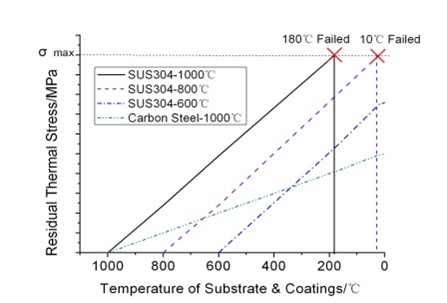
\includegraphics[
      height=0.2\textheight
      ]{figure/subfig1.jpg}
      \subcaption{粗粉涂层}\label{fig:a}
  \end{minipage}
  \begin{minipage}{0.4\linewidth}
    \centering
    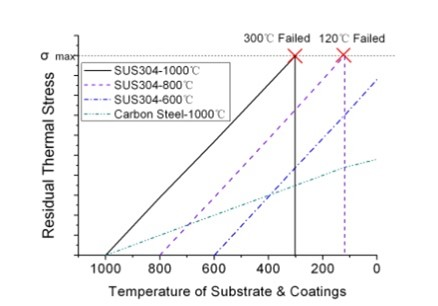
\includegraphics[
      height=0.2\textheight
      ]{figure/subfig2.jpg}
      \subcaption{细粉涂层}\label{fig:b}
  \end{minipage}
  \caption{涂层在冷却过程中残余热应力的变化情况}
  \label{fig:figures}
\end{figure}

\subsection{插图编排}

图的样式必须为嵌入式,居中。插图之前,文中必须有关于本插图的提示,如“见图1.1”、“如图1.1所示”等。插图与其图题为一个整体,不得拆开排写于两页。插图处的该页空白不够排写该图整体时,则可将其后文字部分提前排写,将图移到次页。但是全文的图的编号不能乱,图2.1必须在图2.2之前。有分图时,分图过多在一页内安排不下时,可转到下页,总图题只出现在下页。图与上下正文间需空一行编排。

\section{插入代码块}

尽管在格式要求文件中没有提及,但考虑到代码块的使用比较频繁也比较繁琐,本模板将其一并提供。在本模板中是使用\texttt{listings}宏包插入代码块的,代码块有两种调用形式:

\begin{enumerate}
  \item 在\TeX 中嵌入代码块;
  \item 或以文件形式插入代码。
\end{enumerate}

通过在\TeX 中嵌入代码的形式插入代码块的示例如\ref{lst:insert}所示。

\begin{lstlisting}[language=C, caption={在\TeX 中嵌入代码的形式插入代码块\label{lst:insert}}]
#include <stdio.h>
int main( void ) {
  print("hello, world\n");
  return 0;
}
\end{lstlisting}

以文件形式插入代码块的示例见附录代码\ref{lst:demo}。
    
\section{结论}

根据报告格式要求,“结论”项有如下的格式要求:

\textbf{结论标题}:四号宋体,加粗,顶格,段前20磅,段后10磅,1.25倍行距。

\textbf{结论内容}:宋体小四,段前段后0行,1.25倍行距。

由于上述格式要求并不明确,没有声明“结论”标题的具体位置。但此处“结论”的格式要求实际上与章标题完全一致,因此这里认为结论命令应当居于文档左侧。读者可以使用本模板提供的\texttt{\textbackslash conclusion}命令来生成符合格式要求的“结论”字样。如下展示了一个符合格式要求的“结论”行:

\conclusion

就我们目前所能测定的情况来看,花生酱对地球的自转没有什么影响\cite{PeanutButter}。
 \vspace{0pt}
\chapter{实验步骤与结果}

\section{编译文档}

\subsection{使用make命令编译文档}

如果您习惯使用\texttt{make}命令,并且您的计算机上已经正确配置了GNU Make(譬如基于mingw环境,或者您在大一学习C语言的时候安装过GCC组件作为您的C语言编译器,或者您安装过Git for Windows),那么文档的编译规则已经在Makefile中正确定义。使用\texttt{make}命令能够即刻生成您的文档。

\begin{itemize}
    \item 如果您需要删除工作区目录下包含成品文档在内的所有生成文件,请使用\texttt{make clean}
    \item 如果您只是需要删除所有的辅助文件,请使用\texttt{make clear}
\end{itemize}

\subsection{使用\XeLaTeX 编译文档}

文档需按照如下顺序编译:

XeLaTeX → Biber → XeLaTeX → XeLaTeX

通过在命令行执行如代码\ref{lst:shell_script}所示的命令,你可以正确编译文档:

\begin{lstlisting}[
    language=bash,
    caption={用于编译文档的shell命令}\label{lst:shell_script}]
xelatex main.tex
biber main # 编译引用格式
xelatex main.tex
xelatex main.tex
latexmk -c # 清理工作区
\end{lstlisting} \vspace{0pt}
\chapter{实验总结与心得体会}

\section{帮助完善这篇模板}\label{sec:joinus}

如果您在模板中发现任何不足,欢迎参与模板的改进工作。您可以:

\begin{itemize}
    \item 在本模板的\href{https://github.com/GitHubonline1396529/dlmuucexpreport}{GitHub Repo}提交相应的\href{https://github.com/GitHubonline1396529/dlmuucexpreport/issues}{Issue}/\href{https://github.com/GitHubonline1396529/dlmuucexpreport/pulls}{Pull Request}
    \item 创建模板的Fork。
\end{itemize}

如果你喜欢这个模板,别忘了帮忙点亮Git仓库的小星星。

\section{更新日志}

\begin{itemize}
    \item 2024年7月23日:允许修改封面上的标题和学校名称
    \item 2024年8月1日:修正了章节标题换行的错误;变更文档类型由ctexart为ctexbook
    \item 2024年8月21日:补充说明了有关封面样式差异的问题
    \item 2024年9月13日:修复了封面样式的细微差异;修正了引用文献角标没有方括号的问题。
    \item 2024年9月26日:改进表格字号控制;修正了款项标题编号不显示的问题,改进了款项标题样式。
    \item 2024年10月10日:修正了款项标题的段前段后间距为0行
    \item 2024年10月14日:在文档中新增了文件目录说明,将封面元数据设置迁移至导言区
    \item 2024年10月26日:覆盖了\texttt{maketitle}命令使文档类设计更规范;文档类名称变更
    \item 2024年10月27日:更新了 Makefile 清理辅助文件的逻辑;变更文档类继承为 `report`;兼容 `abstract` 宏包以便用户使用摘要。
    \item 2025年3月14日:将生成封面的逻辑固定到文件\texttt{thecover.sty};在生成的PDF文件的书签目录中显示章节编号;。设置 URL 链接为蓝色;新增若干个 Theorem 环境。
    \item 2025年3月17日:补充文档注释信息。
\end{itemize}
 \vspace{0pt}
\chapter{参考文献}

参考文献按序号、作者、文章题目、期刊名、年份列出;书按序号、作者姓名、书名、出版社、出版时间顺序列出。

\printbibliography[heading=none]

\newpage

\chapter{附录}

\section{宏包}

模板中已加载的宏包如表\ref{tab:packs}所示。请勿重复加载以防止出现问题。

\begin{table}[!h]
    \centering
    \caption{已加载的宏包}\label{tab:packs}
    \begin{tabular}{ccccc}
        \toprule
        ctex & titlesec & array & geometry & fontspec \\
        float & amsmath & amssymb & hyperref & amsthm \\
        mathtools & mathrsfs & calc & tocloft & titletoc \\
        fancyhdr & enumerate & enumitem & metalogo & setspace \\
        caption & subcaption & booktabs & multirow & longtable \\
        chemfig & tikz & tikz-network & circuitikz & color \\
        xcolor & verbatim & listings & matlab-prettifier &  \\
        \bottomrule
        \end{tabular}
\end{table}

\section{插入代码块效果示例}

\lstinputlisting[
    language=Python, 
    caption={系统聚类方法的实现(Python):\label{lst:demo}} 
    ]{code/demo.py} % Python

 \vspace{0pt}

\end{document}